%!TEX root = Thesis.tex

\chapter{Methodology}
\label{chapter:methodology}


%TODO explain methodology to obtain results of quantum clustering of just present results on why it was not viable?

%TODO This is where I explain my approach to the problem of EAC in Big Data

The aim of this thesis is the optimization and scalability of EAC, with a focus for large datasets.
EAC is divided in three steps and each has to be considered for optimization.

The first step is the accumulation of evidence, i.e. generating an ensemble of partitions.
The main objective for the optimization of this step is speed.
Using fast clustering methods for generating partitions is an obvious solution, as is the optimization of particular algorithms aiming for the same objective.
Since each partition is independent from every other partition, parallel computing over a cluster of computing units would result in a fast ensemble generation.
Using either or any combination of these strategies will guarantee a speed-up.

Initial research was under the field of quantum clustering.
After this pursuit proved fruitless regarding one of the main requirements (speed), the focus of researched shifted to parallel computing, more specifically a K-Means parallel version within the GPGPU paradigm.
	
The second step is mostly bound by memory.
The complete co-association matrix has a space complexity of $\mathcal{O}(n^2)$.
Such complexity becomes prohibitive for big data, e.g. a dataset of $2 \times 10^6$ samples will result in a complete co-association matrix of $14901 \; GB$ if values are stored in single floating-point precision.
%This work was focused on sparse matrices.% and cutting associations.
This problem is addressed by exploring the inherent sparse nature of the co-association matrix.

The last step has to take into account both memory and speed requirements.
The final clustering must be able to produce good results and be fast while not exploding the already big space complexity from the co-association matrix.
The work in this last step was initially directed towards parallelization and afterwards out-of-core processing using a disk stored co-association matrix.% and sparse matrices.

The methodology for optimizing for speed is relevant and permeates the approach taken to every problem faced in the present work.
For optimizing the speed of an algorithm, one starts by first profiling said algorithm and analyze which parts take the longest to compute.
These parts are the focus of optimization as any change on them will have the greatest effect on the overall algorithm.
To further illustrate this point, let us consider an algorithm that spends 75\% on a section of the code to which a speed-up of $2$ is possible and 25\% on a part to which an infinite speed-up is possible (this translates in its execution time being negligible).
Let us further assume that only one part of the algorithm may be optimized.
If one optimizes the first part, the local speed-up is $2$ and the overall speed-up is $1.6$.
On the other hand, if one optimizes the second part, the local speed-up is infinite but the overall speed-up is only $1.333(3)$.
%refer Amdhal Law? it is formally more oriented torwards parallel computing and number of threads

All the algorithms were implemented in Python with high reliance on numerical and scientific modules, namely NumPy \cite{VanDerWalt2011} and SciPy \cite{JonesSciPy,Oliphant2007,Millman2011}.
Important modules for visualizing and processing statistical results were MatplotLib \cite{hunter2007matplotlib} and Pandas \cite{McKinney2010}, respectively.
The SciKit-Learn \cite{Pedregosa2012} machine learning library has a plethora of implemented algorithms which were used for benchmarking as well as integration in the devised solutions.
The iPython \cite{Perez2007} module was used for interactive computing which allowed for accelerated prototyping and testing of algorithms.
Python is a interpreted language which translates in its performance being worse than a compiled language such as C or Java.
To address this problem, the open-source Numba module from Continuum Analytics was used to allow for writing code in native Python and have it converted to fast compiled code.
Furthermore, this module provides a pure Python interface for the CUDA API.
The proprietary NumbaPro module was used for two high level CUDA functions, namely \emph{argsort} and \emph{max}. %TODO write this one a bit better


\section{Quantum Clustering}

Research under this paradigm aimed to find a candidate for the first phase of EAC.
Two candidates were considered: Quantum K-Means (QK-Means) and Horn and Gottlieb's quantum clustering (QC)algorithm.
These algorithms were chosen so as to have a representative from both approaches identified in chapter \ref{chapter:stateofart}.


The implementation QK-Means followed the description presented in section \ref{sec:qkmeans}, with the exception of the genetic operations \emph{cross-over} and \emph{mutation}.
This change was made because literature \cite{Liu2010} suggested that enough variability is produced in the quantum rotation step with the angle-distance rotation method.
Furthermore, the main goal for the first phase of EAC is speed but these operations aim at improving the quality of the solution.
As such, it was an implementation decision to cut overhead where possible since literature supported that no significant changes would affect the final result.

An implementation of QC was already available in Matlab.
Accordingly, implementing this algorithm translated into porting the code from Matlab to Python.

% For both, the experiments that were setup had the goal of evaluating the speed and accuracy performances of the algorithms.


% This should be 
% Under the qubit concept, no other algorithms were experimented with since the results for this particular algorithm showed that this kind of approach is infeasible due to the cost in computational speed.
% The results highlight that fact.

\section{Speeding up Ensemble Generation with Parallel K-Means}

K-Means is an obvious candidate for the generation of partitions since it is simple, fast and partitions do not need to be accurate - variability in the partitions is a desirable property.
This relaxation on the accuracy of the partitions already allows for a faster generation of partitions since fewer iterations of the algorithm need to be executed for a partition to be generated - typically 3 iterations suffice.
Further gains are possible with a parallel GPU version of K-Means.
The overview of the algorithm used is presented in section \ref{sec:parallel kmeans}.
This section will offer implementation details.

The implementation gives as much freedom as possible to the user regarding CUDA parameter choices.
By default, each thread will compute the label of one pattern and the blocks are unidimensional and composed by 512 threads.
The number of blocks, then, is the number of patterns divided by the the number of threads per block.
If the number of blocks exceeds the maximum allowed for one dimension (65535), the grid configuration automatically uses other dimensions.
The other parameter that the user can choose deals with how data is transfered back and forward between host and device.
The user can choose to allow the CUDA API to handle all the memory transfers or to make the implementation optimize those.
The latter will minimize the amount of data transfers and memory allocations and is the default option.
Furthermore, it also allows for the algorithm to be executed multiple times without redundant transfer of the pattern set.
This permits for the production of an entire ensemble with a single transfer of the pattern set.
These parameters (number of patterns per thread, number of threads per block and memory transfer mode) may be configured at runtime.
Still, a typical user does not need to be knowledgeable about CUDA to be able to use this implementation, since the tuning of these parameters is optional.

The CUDA implementation of the label computation part of the algorithm starts by transfering the data to the GPU (pattern set and initial centroids) and allocates space for the labels and corresponding distances.
The computation of a label for one pattern is done by iteratively computing the distance from the pattern to each centroid and storing the label and the distance corresponding to the closest centroid to that pattern.
Finally, the labels and distances are sent back to the host for computation of the centroids.
This procedure is available as a CUDA kernel or as three different sequential versions: pure Python, based on NumPy or compiled code with Numba.
These same sequential versions exist for the recomputation of the centroids.
The implementation of the centroid computation starts by counting the number of patterns attributed to each centroid.
Afterwards, it checks if there are any "empty" clusters, i.e. if there are centroids that are not the closest ones to any pattern.
Dealing with empty clusters is important because, although empty clusters may be desirable in some situations, the target use expects that the output number of clusters to be the same as defined in the input parameter.
Centroids corresponding to empty clusters will be the patterns that are furthest away from their centroids.
Any other centroid $c_i$ will be the mean of the patterns that were labeled $i$.


%TODO pseudocode & diagrams

\section{Dealing with the space complexity of the co-association matrix}

In chapter \ref{chapter:stateofart}, two approaches to the space complexity of the co-association matrix in the second phase of EAC are presented: one dealing with $p$ prototypes and the other with the inherent sparsity of the matrix. 

The results presented in the sparsity study of EAC \cite{Lourenco2010} show that it is possible to obtain a high sparsity in the co-association matrix.
In some comes the density of the matrix was as low as 1\%.
This motivated the focus of the work on exploiting the inherent sparsity of the matrix.
A discussion on using sparse matrices and a novel solution for building the co-association matrix is presented \ref{sec:sparse coassoc}.

As stated before, the focus of the work is on sparse matrices.
Still, for the sake of completeness, the different strategies considered for the prototypes approach are discussed here.
One strategy is to use the \textbf{p-Nearest Neighbors} as prototypes, as already presented in chapter \ref{chapter:stateofart}.
Before building the co-association matrix, the $p$ closest samples to each sample are computed and stored in the $n \times p$ neighbor matrix.
During the voting mechanism of EAC only the neighbors of each pattern are considered.
This strategy has a space complexity of $O(2nk)$ and requires the computation of the k-Nearest Neighbors.
A second strategy is to use \textbf{p random prototypes}, which will a set of unique $p$ patterns.
This will be the same for every sample.
Here the voting mechanism is altered so that if a sample is clustered with any of the prototypes, the correspondent element in the co-association matrix is incremented.
This has the advantage that only a $n \times p$ matrix needs to be stored along with a $p$ array for the chosen prototypes.
Furthermore, if $p$ if high enough to provide a representative sample of the dataset the results can be as good as the full matrix.
The third, and final, possible strategy identified is similar to the random prototypes.
The difference is that instead of choosing $p$ random samples from the dataset, the prototypes will be the representatives of the dataset from another algorithm, e.g. K-Medoids, K-Means.

It would be ideal to combine both approaches (sparsity and neighbors) to further reduce space complexity, but they are not necessarily compatible.
This is specially true for the p-Nearest Neighbors strategy since it is unlikely that a sample will never be clustered with its closest $p$ neighbors.
This means that the $n \times p$ co-association matrix may not have many zeros which translates in little advantage for using the sparsity augmentation approach the matrix of co-associations.
% Still, one should note that the p-Nearest Neighbors strategy is closely related to a sparse representation.
% these seem more like comments for results.
% Still, this highly depends on the the number of neighbors relative to the number of samples and also the granularity of the partitions.
% If the number of neighbors is high, one of the neighbors can be sufficiently far away from the sample to not clustered with it.
% If the granularity of the partitions is high (i.e. there are a high number of small clusters) then each cluster may have sufficiently few samples that neighbors are not included.

\section{Building the sparse matrix}
\label{sec:sparse coassoc}

Building a non-sparse matrix is easy and fast since the memory for the whole matrix is allocated and indexing the matrix is direct.
When using sparse matrices, neither is true.
In the specific case of EAC, there is no way to know what is the number of associations the co-association matrix will have which means it is not possible to pre-allocate the memory to the correct size of the matrix.
This translates in allocating the memory gradually which may result in fragmentation, depending on the implementation, and more complex data structures, which incurs overhead.

% Several sparse matrices exist
% some are better for building others for computing
% describe my solution

Documentation of the SciPy library recommends different sparse formats for either building a matrix or operating over it.
For building a matrix, the COO (COOrdinate), DOK (Dictionary of Keys) and LIL (List of Lists) formats are recommended.
All of these formats rely on extra data structures such as lists as dictionaries to efficiently build the matrices incrementally, i.e. allocating memory as it is required.
For operating over a matrix, the documentation recommends converting from one of the previous formats to either CSR (Compressed Sparse Row) or CSC (Compressed Sparse Column).

%TODO insert real times from small simulation
As observed before, the sparsity study of EAC \cite{Lourenco2010} did not account for the overhead of using the data structures supporting sparse matrices.
However, scaling to very large data sets must take this into account.
Exploratory testing revealed that using one of the recommended matrices allowed for building the matrix took around two orders of magnitude as long as using a full allocated matrix.
Furthermore, because of the extra data structures, the implementations from SciPy would saturate the main memory from data sets with less than 1 million patterns.
Using the CSR format did not saturate memory but it took a completely unacceptable amount of time, many orders of magnitude above any of the formats recommended for building the matrix.

After a search in the literature for efficient and scalable ways to build a sparse matrix proved fruitless, this issues motivated the design of a new method for building the matrix specialized for the characteristics of EAC.
The solution devised is based on the CSR format, which has the desired properties of having a low memory trace and allows for fast computations.

\subsection{EAC CSR}

The first step is making an initial assumption on the maximum number of associations \emph{max\_assocs} that each sample can have.
A possible rule is $$max\_assocs = 3 \times bgs$$ where $bgs$ is the biggest cluster size in the ensemble.
The biggest cluster size is a good heuristic for trying to predict the number of associations a sample will have since it is the limit of how many associations each sample will have in any partition.
Furthermore, one would expect that the neighbors of each sample will not vary significantly, i.e. the same neighbors will be clustered together with a sample repeatedly in many partitions.
This scheme for building the matrix uses 4 supporting arrays:

\begin{itemize}
	\item \textbf{indices} - an array of $n \times max\_assocs$ size that stores the columns of each non-zero value of the matrix, i.e. the destination sample to which each sample associates with;
	\item \textbf{data} - an array of $n \times max\_assocs$ size that stores all the non-zero values;
	\item \textbf{indptr} - an array of $n$ size where the \emph{i-th} element is the pointer to the first non-zero value in the \emph{i-th} row.
	\item \textbf{degree} - an array of $n$ size that stores the number of non-zero values of each row.
\end{itemize}

Each sample (row) has a maximum of \emph{max\_assocs} pre-allocated that it can use to fill with new associations.
New associations that exceed this pre-allocated maximum are discarded.
%Since each sample has a maximum pre-defined number of associations, \emph{indptr} does not really need to exist since it can be easily deduced (e.g. $indices[n] = n \times max\_assocs$).
The \emph{degree} array is the one keeping track of the number of associations of each sample.
Throughout this section, the interval of the \emph{indices} array corresponding to a specific pattern (row) is referred to as the \emph{indices} interval.
If it is said that an association is added to the end of the \emph{indices} interval, this refers to the beginning of the part of the interval that is free for new associations.
Furthermore, it should be noted that this method assumes that the clusters received come sorted in a increasing order.

The first partition is inserted in a special way.
Since it is the first and the clusters are sorted, it is a matter of copying the cluster to the \emph{indices} array in the positions of each sample, with the exclusion of the sample itself.
The data array (containing the co-association score) is set to 1 on the relevant positions.
This process can be observed clearly in Fig. \ref{fig:first part}.
Because it is the fastest partition to be inserted, it is picked to be the one with the least amount of clusters (more samples per cluster) so that each sample gets the most amount of associations in the beginning (on average).
This is only applicable if the whole ensemble is provided, otherwise there is no way to know what is the biggest cluster of the whole ensemble.
This increases the probability that any new cluster will have more samples that correspond to already established associations.
Because the clusters are sorted and only a copy of each cluster was made, it is not necessary to sort each row of the matrix by column index.

\begin{figure}[hbtp]
\centering
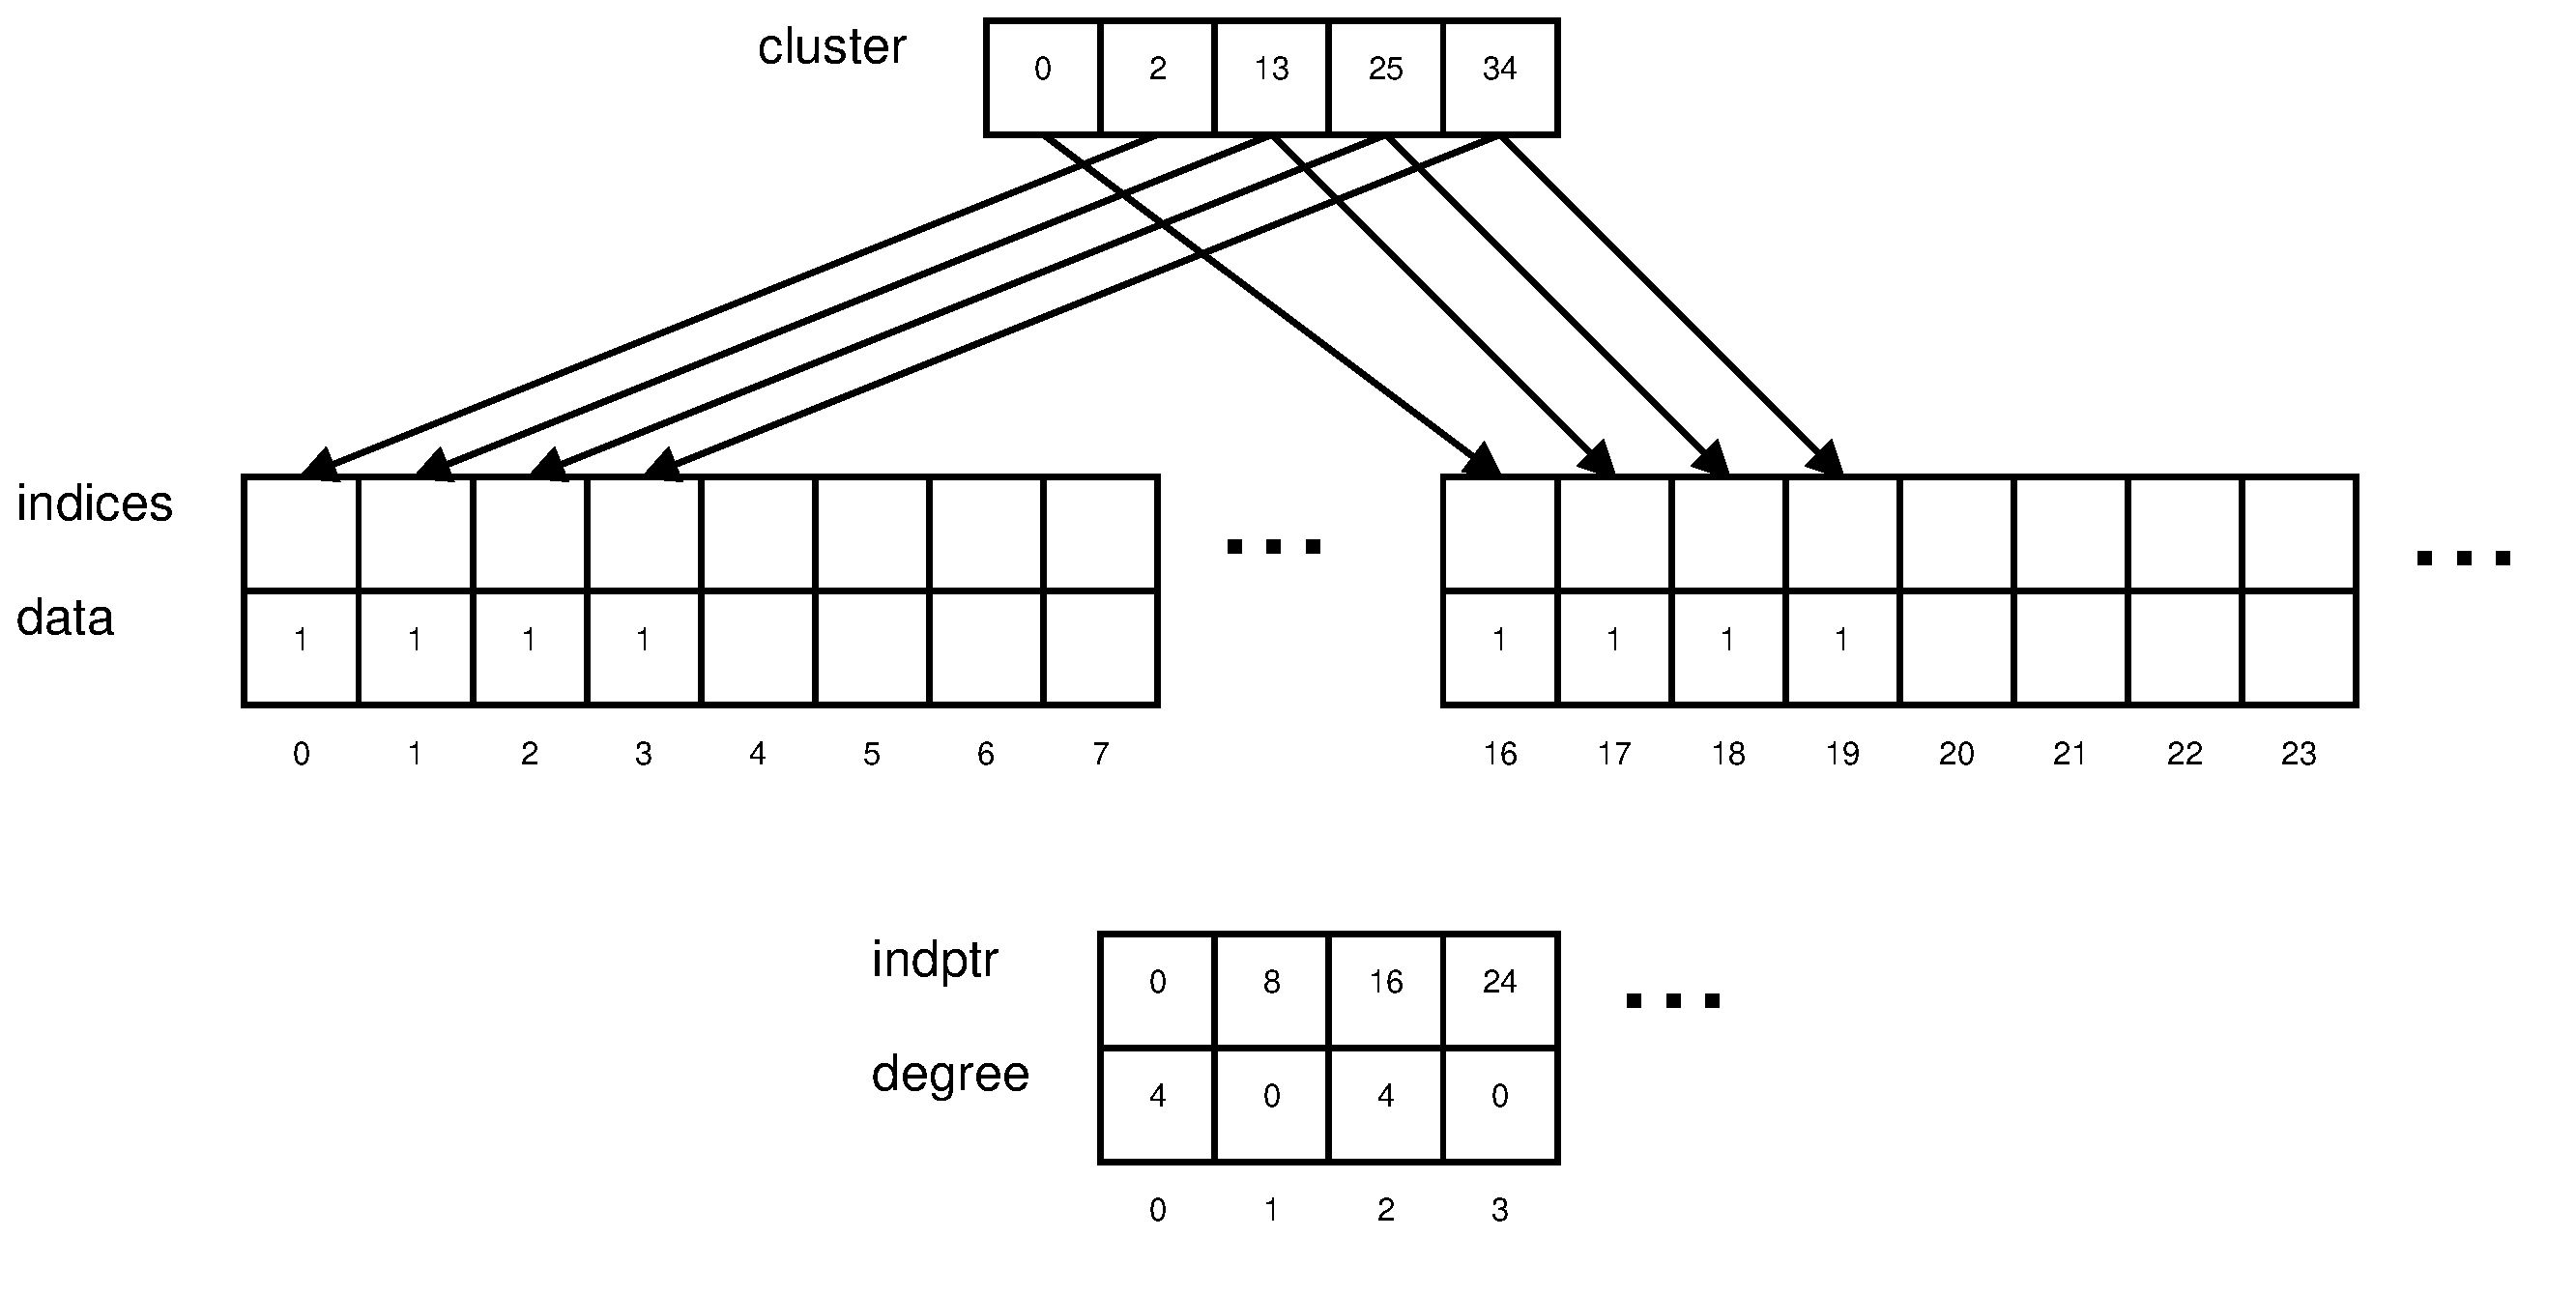
\includegraphics[width=\textwidth]{methodology/eac_csr_first_part}
\caption{Inserting a cluster of the first partition in the co-association matrix.}
\label{fig:first part}
\end{figure}

For the remaining partitions, the process is different.
Now, it is necessary to check if an association already exists.
For each sample in a cluster it is necessary to add or increment the association to every other sample in the cluster.
This is described in Algorithm \ref{alg:eac csr update cluster}.


\begin{algorithm}
\caption{Update matrix with cluster.}\label{alg:eac csr update cluster}
\begin{algorithmic}[1]
\Procedure{update\_cluster}{$indices, data, indptr, degree, cluster, max\_assocs$}
\For{$sample$ $\mathbf{n}$ $in$ $cluster$}
	\For{$every$ $other$ $sample$ $\mathbf{na}$ $in$ $cluster$}
		\State{$ind$ $=$ $binary\_search(na, indices,$$interval$ $of$ $n$ $in$ $indices)$}
		\If{$ind \ge 0$}
			\State{$increment$ $data[ind]$}
		\Else
            \If{$maximum$ $assocs$ $not$ $reached$}
			    \State{$add$ $new$ $assoc.$ $with$ $weight$ $1$}
            \EndIf
		\EndIf
	\EndFor
\EndFor
\EndProcedure
\end{algorithmic}
\end{algorithm}

The binary search is used to search for the association in the indices array in the interval corresponding to a specific row (or pattern).
This is necessary because it is not possible to index directly a specific position of a row in the CSR format.
Since a binary search is performed $(ns - 1)^2$ times for each cluster, where $ns$ is the number of samples in any given cluster, the indices of each sample must be in a sorted state at the beginning of each partition insertion.
Two strategies for sorting were devised.
The \underline{first strategy} is to just insert the new associations at the end of the \emph{indices} array (in the correct interval for each sample) and then, at the end of processing each partition, use a sorting algorithm to sort all the samples' intervals in the \emph{indices} array.
This was easily implemented with existing code, namely using \emph{NumPy}'s \emph{quicksort} implementation, which has an average time complexity of $O(n \log n)$

The \underline{second strategy} is more complex.
It results from the observation that, if one could know in which position each new association should be inserted, it would be possible to move all old associations to their final sorted positions and insert the new ones.
Furthermore, this would be done in an efficient manner with minimum number of comparisons (and thus branches in the execution of the code).
For this end, the implemented binary search returns the index of the searched value (key) if it is found or $-ind -1$, where $ind$ is the position for a sorted insertion of the key in the array, if it is not found.
This means that the position where each new association should be inserted is now available.
Instead of just adding the new associations after the old ones of each sample, new associations are stored in two auxiliary arrays of size $max\_assocs$: one (\emph{new\_assoc\_ids}) for storing the patterns of the associations and the other (\emph{new\_assoc\_idx}) to store the indices where the new associations should be inserted (the result of the binary search).
The process is illustrated with an example in Fig. \ref{fig:normal part}, detailed in Algorithm \ref{alg:eac csr sort cluster} and explained in the following paragraph.

After each pass on a cluster (adding or incrementing all associations to a sample in the cluster), the new associations have to be added to the pattern's indices interval in a sorted manner.
The number of associations corresponding to the $i$-th pattern (\emph{degree[i]}) is incremented by the amount of new associations to be added.
%The new interval of the \emph{indices} array belonging to the $i$-th sample now has \emph{degree[i]} plus the number of new associations.
An element is added to the end of the \emph{new\_assoc\_idx} array with the value of \emph{degree[i]} so that the last new association can be included in the general cycle.
During the sorting process a pointer to the current index to add associations $o\_ptr$ is kept ( it is initialized to the new total number of associations of a sample).
The sorting mechanism looks at two consecutive elements in the \emph{new\_assoc\_idx} array, starting from the end.
If the $i$-th element of the \emph{new\_assoc\_idx} array is greater or equal than the $(i-1)$-th element, then all the associations in the \emph{indices} array between them (including the first element) are copied to the end of the \emph{indices} interval, i.e. they are shifted to the right by $i$ positions.
Then, or in case the comparison fails, the $(i-1)$-th element of the \emph{new\_assoc\_ids} is copied to the \emph{indices} array in the position specified by \emph{o\_ptr}.
The \emph{o\_ptr} pointer is decremented anytime an association is written in the \emph{indices} array.

% TODO check which or the three fast sorting approaches is best and describe only that one

\begin{figure}[hbtp]
\centering
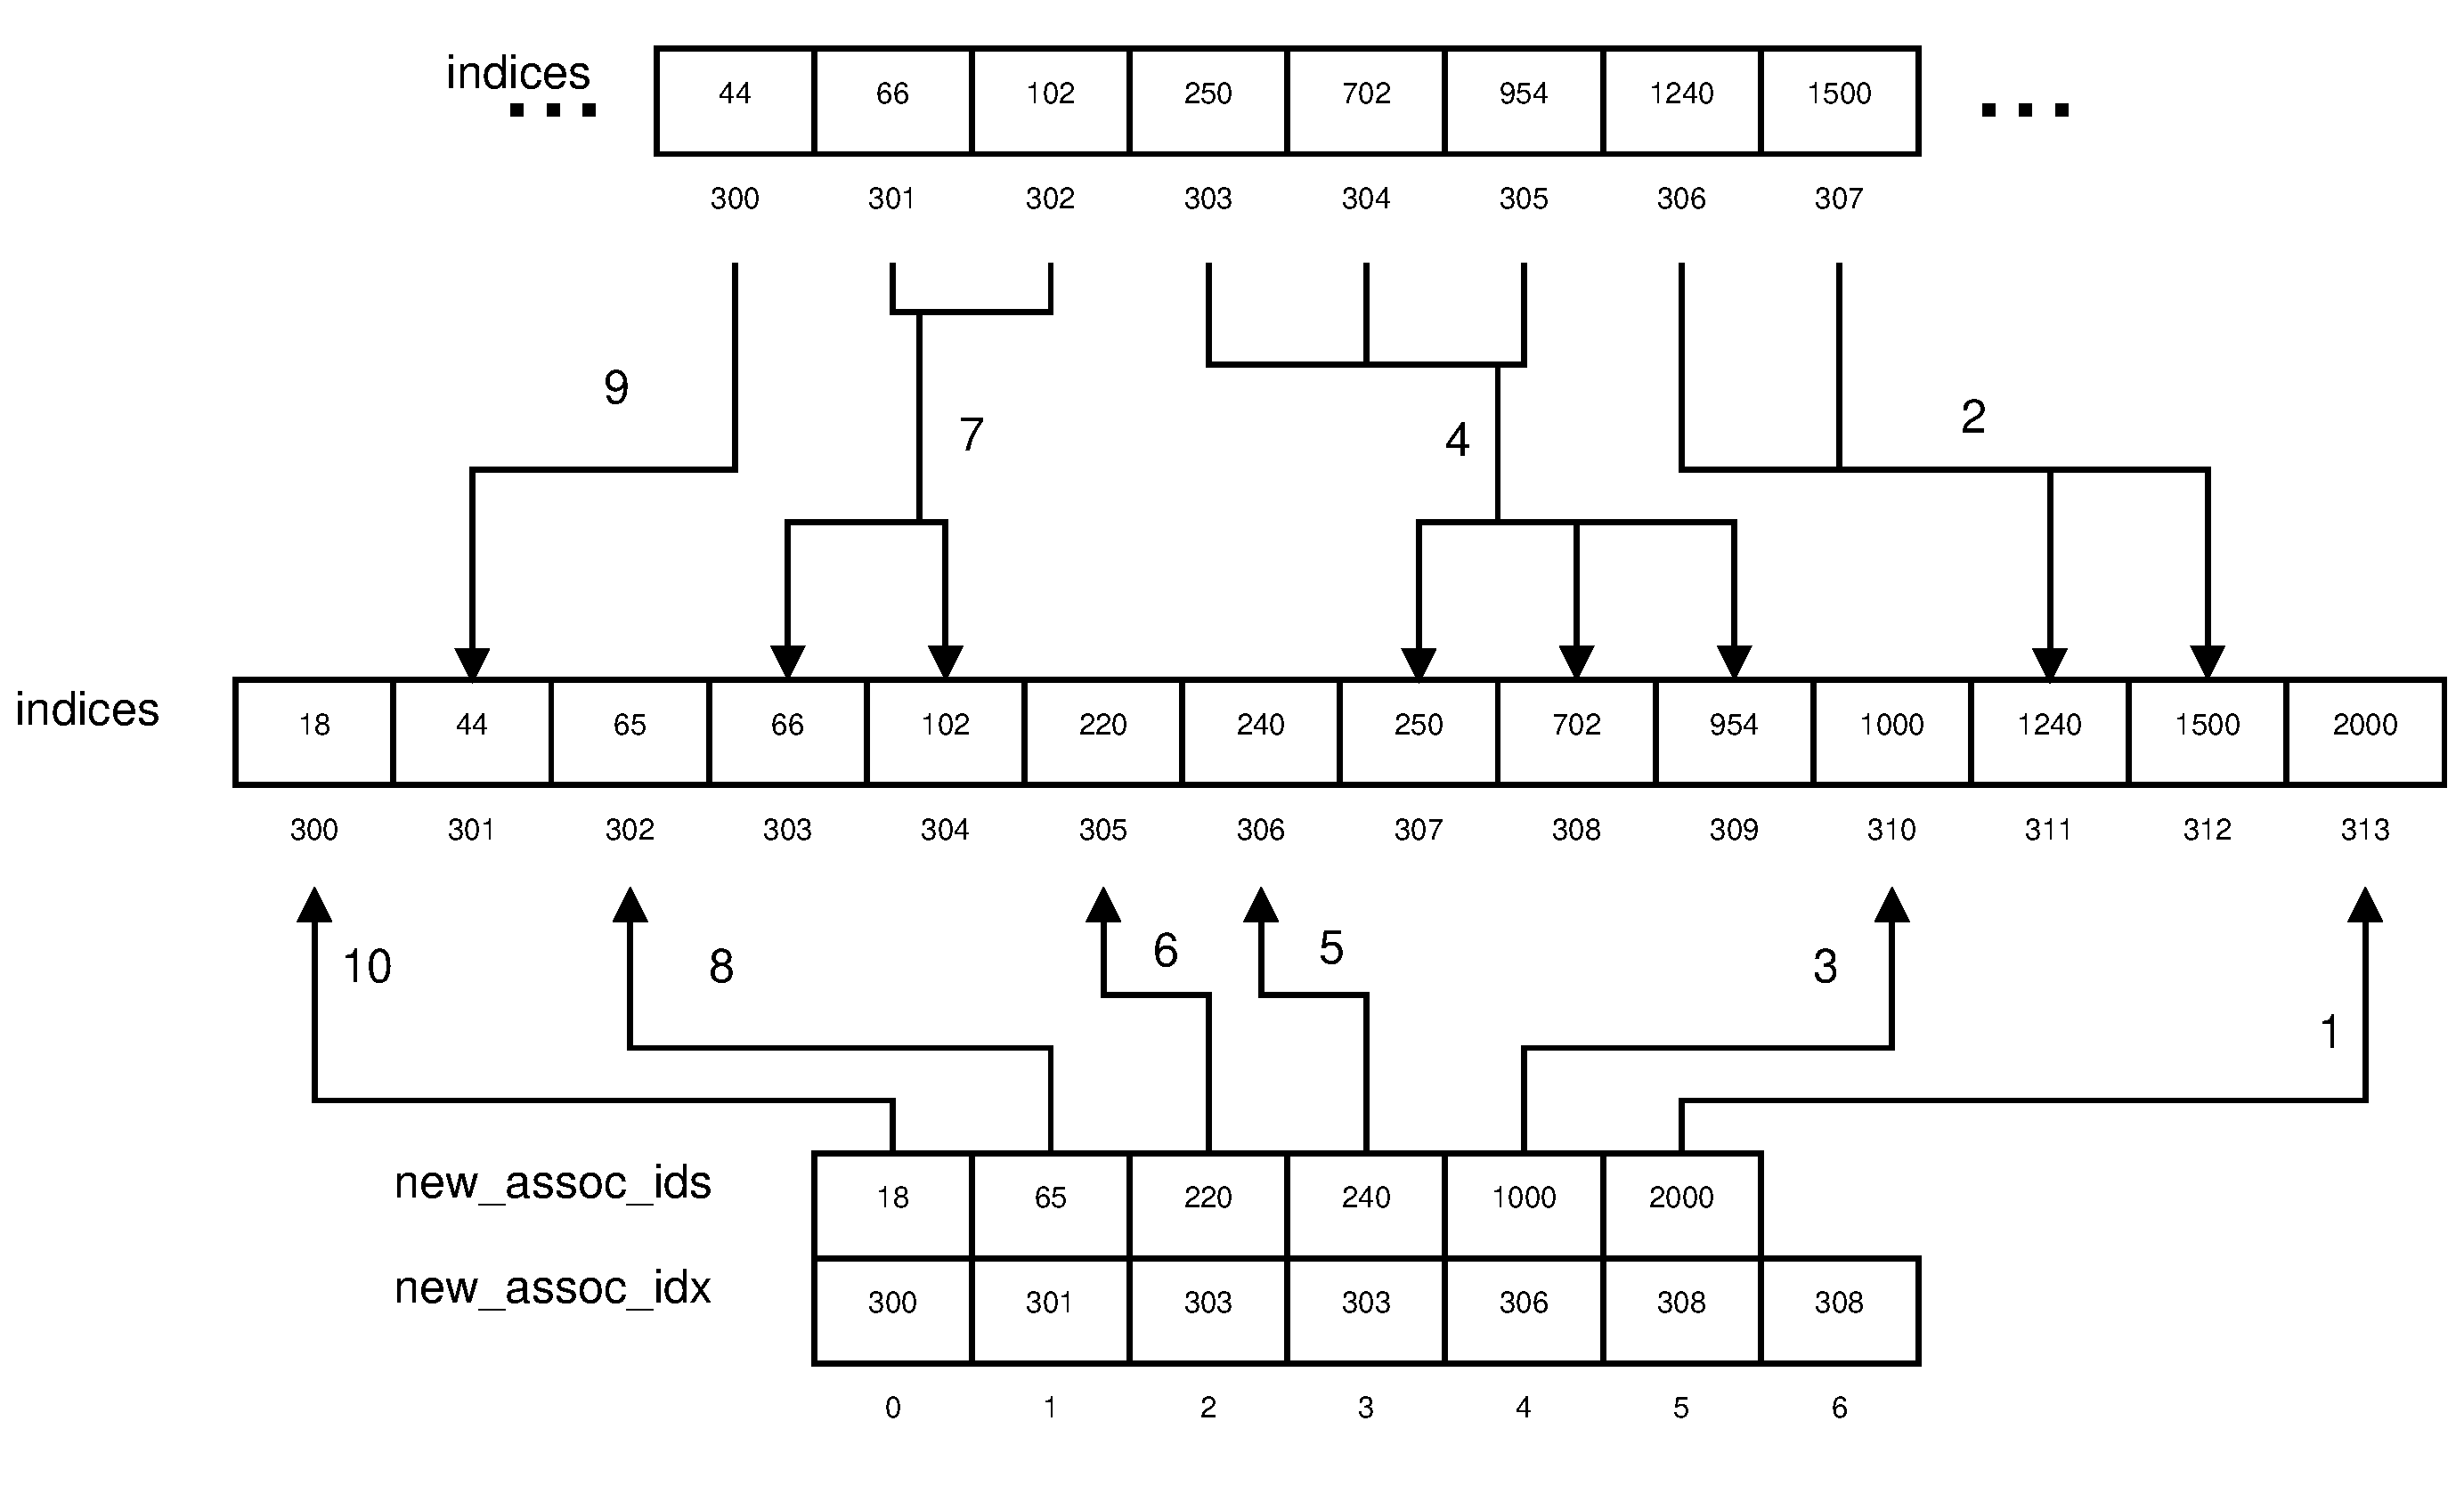
\includegraphics[width=\textwidth]{methodology/sorted_insert}
\caption{Inserting a cluster from a partition in the co-association matrix. The arrows indicate to where the indices are moved. The numbers indicate the order of the operation.}
\label{fig:normal part}
\end{figure}



\begin{algorithm}
\caption{Sort the \emph{indices} array in the interval of a sample $n$.}\label{alg:eac csr sort cluster}
\begin{algorithmic}[1]
\Procedure{sort\_indices}{$indices, data, indptr, degree, n, new\_assocs\_ptr, new\_assocs\_ids, new\_assocs\_idx$}
\State{$new\_assocs\_idx[new\_assocs\_ptr] = indptr[n] + degree[n]$}
\State{$i = new\_assocs\_ptr$}
\State{$o\_ptr = indptr[n] + new\_assocs\_ptr + degree[n] - 1$}
\While{$i \ge 1$}
	\State{$start\_idx = new\_assocs\_idx[i - 1]$}
	\State{$end\_idx = new\_assocs\_idx[i] - 1$}

    \While{$end\_idx >= start\_idx$}
        \State{$indices[o\_ptr] = indices[end\_idx]$}
        \State{$data[o\_ptr] = data[end\_idx]$}
        \State{$end\_idx -= 1$}
        \State{$o\_ptr -= 1$}
    \EndWhile
    \State{$indices[o\_ptr] = new\_assocs\_ids[i - 1]$}
    \State{$data[o\_ptr] = 1$}    
    \State{$o\_ptr -= 1$}
    \State{$i -= 1$}
\EndWhile

\EndProcedure
\end{algorithmic}
\end{algorithm}

\subsection{EAC CSR Condensed}

The co-association matrix is symmetric, which means that only half is necessary to describe the whole matrix.
That fact has consequences on both memory usage and computational effort on building the matrix.
In the case of the fully allocated matrix, this translates in a reduction to 49.5\% of the memory required.
Furthermore, only half the operations are made since only half the matrix is accessed, which also accelerates the building of the matrix.
There is, however, a small overhead for translating the two dimensional index to the single dimensional index of the upper triangle matrix.
When using a sparse matrix according to the EAC CSR scheme described above, there is no direct memory usage reduction.
However, the number of binary searches performed by inserting new associations is half which has a significant impact on the computation time relative to the complete matrix.

Even though there is no direct memory reduction for switching to the condensed matrix form, this scheme does open possibilities for it.
Previously, the number of associations for each sample (number of non zero values in each row) remained constant throughout the whole set of patterns.
However, using a condensed scheme means that the number of associations decreases as one steps further to the end of the set, i.e. closer to the bottom the co-association matrix.
An example of this can be seen in the plot of the number of associations per sample in a complete and condensed matrix of Fig. \ref{fig:coassoc degree}.
It is clear that, since the number of associations that is actually stored in the matrix decreases throughout the matrix, the pre-allocated memory for each sample can decrease accordingly.
One possible strategy, illustrated in Fig. \ref{fig:coassoc degree}, is to decrease the maximum number of associations linearly.
In the example, the first 5\% of samples have the 100\% of the maximum number of associations and it decreases linearly until 5\% of the maximum number of associations for the last sample.

Table \ref{tab:mat type memory} shows the memory usage of the different co-association matrix strategies in the general case and for an example of 100000 patterns.
The memory consumption for the \emph{sparse condensed linear} type of matrix if given for the parameters presented above for Fig. \ref{fig:coassoc degree}.

\begin{table}[hbtp]
\centering
\caption{Memory used for different matrix types for the generic case and a real example of 100000 samples. The relative reduction (R.R.) refers to the memory reduction relative to the type of matrix above, the absolute reduction (A.R.) refers to the reduction relative to the full complete matrix.}
\label{tab:mat type memory}
\begin{tabular}{lrrrr}
\toprule
\textbf{Type of matrix}          & \textbf{Generic}                & \textbf{Memory {[}MBytes{]}}    & \textbf{R.R.} & \textbf{A.R.} \\
\midrule% \hline
Full complete           & $N^2$                  & $9536.7431$              & -                  & -             \\
Full condensed          & $\frac{N(N-1)}{2}$     & $4768.3238$              & $0.4999$     & $0.4999$      \\
Sparse constant         & $ 0.54 \times N \times max\_assocs$ & $678.8253$               & $0.1423$           & $0.0711$      \\
Sparse condensed linear & $N \times max\_assocs$ & $372.8497$               & $0.5492$           & $0.0390$      \\
\bottomrule
\end{tabular}
\end{table}


\begin{figure}[hbtp]
\centering
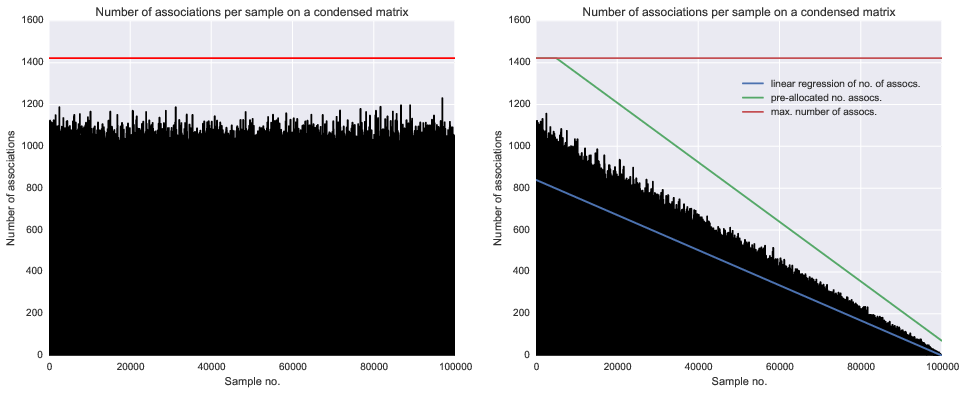
\includegraphics[scale=0.45]{methodology/eac_csr_cond_full_degree_100k}
\caption{The left figure shows the number of associations per sample in a complete matrix; the right figure shows the number of associations per sample in a condensed matrix.}
\label{fig:coassoc degree}
\end{figure}


\section{Final partition recovery}

This section will present the considered candidates for the final step of EAC.
A GPU version of SL is described in section \ref{sec:sl gpu}.
External algorithms are a candidate solution and this approach is presented in section \ref{sec:sl disk}.
This solution is based on storing the co-association matrix on disk, performing the expensive computation (memory and speed wise) of \emph{argsort} and then processing the matrix in batches until the final MST is extracted.

\subsection{Single-Link and GPGPU}
\label{sec:sl gpu}
% introduction to the procedure of SL with MST
Single-Link is an inherently sequential algorithm which means an efficient GPU version is hard to implement.
However, SL can be performed by computing the MST and cutting edges until we have the desired number of clusters, as described in chapter \ref{chapter:stateofart}.
Considerable speed-ups are reported in the literature for MST solvers in the GPGPU paradigm.
The considered solution uses the efficient parallel variant of Borůvka's algorithm \cite{Sousa2015}.
After the necessary pruning of the MST edges has been performed to achieve the desired number of clusters, the output MST is fed to the labeling algorithm which will provide the final clustering.

\subsubsection{Generating the MST}
% explain modification to the MST algorithm to accept unconnected graphs
The output of the Borůvka's algorithm is a list of the indices of the edges constituting the MST. 
These indices point to the \emph{destination} of the original graph. 
The original algorithm \cite{Sousa2015} assumes connected graphs, but this is not guaranteed in EAC's co-association matrix.
In graph theory, given a connected graph $G = (V,E)$, there is a path between any $s,t \in V$, where $V$ is the set of vertices in $G$ and $E$ is the set of edges that connects the vertices.
In an unconnected graph, this is not the case and unconnected subsets are called components, i.e. a connected component $C \subset V$ ensures that for each $u,v \in C$ there is a path between $u$ and $v$.
In the present implementation, the issue of unconnected graphs was solved in the first step (finding the minimum edge connected to each vertex or supervertex). 
If a vertex has no edges connected to it (an outdegree of 0 since all edges are duplicated to cover both directions) then it is marked as a mirrored edge. 
This means that the independent components will be marked as supervertices in all subsequent iterations of the algorithm. 
The overhead of having these redundant vertices is low since the number of independent components is typically low compared to the number of vertices in the the graph and the processing of such vertices is very fast.
As a consequence, the stopping criteria becomes the lack of edges connected to the remaining vertices, which is the same as saying that all elements of the \emph{outdegree} array are zero. 
This condition can be checked as a secondary result of the computation of the new \emph{first\_edge} array. 
This step is performed by applying an exclusive prefix sum over the \emph{outdegree}. 
The prefix sum was implemented in such a way that it returns the sum of all elements, which translates in very low overhead to check this condition.
The final output is the MST array and the number of edges in the array. 
The later is necessary because the number of edges will be less than $|V|-1$ when independent components exist, and also because the MST array is pre-allocated in the beginning of the algorithm when the number of edges is not yet known.

\subsubsection{Number of clusters and pruning the MST}
% cutting edges
The number of clusters can be automatically computed with the lifetime technique or be supplied. 
Either way, a list (\emph{mst\_weights}) with the weights of each edge of the MST is compiled and ordered.
The list of edges is also ordered according to the order of the \emph{mst\_weights}. 
If the number of clusters $k$ was given, the algorithm removes the $k - 1$ heaviest edges. 
If there are independent components inside the MST those are taken into consideration before removing any edges.
If the number of clusters $k$ is higher than the number of independent components the final number of clusters will be the number of independent components.

To compute the number of clusters (which results in a truly unsupervised method) the lifetimes are computed.
In the traditional EAC, lifetimes are computed on the weights of the clusters by the order they are formed.
With the MST, the lifetimes are computed over the ordered \emph{mst\_weights} array, which is equivalent.
If there are independent components, an extra lifetime is computed from the representative weight connecting independent components.
This lifetime will serve as the threshold between choosing the number of independent components as the number of clusters or looking into the lifetimes within the MST.
This is because links between independent vertices are not included in the MST.
For this reason, the lifetime for going from independent edges to the heaviest link in the MST (where the first cut would be performed) is computed separately.
If the maximum lifetime within the MST is bigger than the threshold, than the number of clusters is computed as in traditional EAC plus the number of independent components.
Otherwise, the independent components will be the final clusters.
Most of this process can be done by the GPU.
Library kernels were used to sort the array and compute the $arg max$, and a simple kernel was used to compute the lifetimes.

\subsubsection{Building the new graph}
The final MST (after performing the pruning) is then converted into a new, reduced graph.
The function responsible for this takes the original graph and the final selection of edges that composing the MST and, afterwards, produces a graph in CSR format.
The function has to count the number of edges for each vertex, compute the origin vertex of each edge (the original \emph{destination} array only contains the destination vertices) and, with that information, build the final graph.
This process can be done by the GPU with simple mapping kernels and a modified binary search for determining the origin vertex.

\subsubsection{Final clustering}
The last step is computing the final clusters.
Any incision in the MST translates in independent components in the constructed graph.
This means that the problem of computing the clusters translates into a problem of finding independent connected components in a graph, a problem that usually goes by the name of Connected Component Labeling.
To implement this part in the GPU, the aforementioned Borůvka algorithm was modified to output the an array \emph{labels} of length $|V|$ such that the $i-th$ position contained the label of the $i-th$ vertex.
To this effect, the flow of the algorithm was slightly altered as shown in Figure \ref{fig:connected comps flow}. 
The kernel dealing with the MST was removed and a kernel to update the labels at each iteration, shown in Algorithm \ref{alg:comp_labels}, was implemented.
In the first iteration of the algorithm the converged colors are copied to the labels array.
In every iteration the kernel to update the labels takes in the propagated colors and the array with the new vertex IDs.
For each vertex in the array, the kernel first takes in the the color of the current vertex and maps it to the new color (one should notice that the color is actually a vertex ID and that that vertex has had its color updated).
Afterwards, the kernel maps the new color with the new vertex ID that color will take, to keep consistency with future iterations.

\begin{figure}[hbtp]
\centering
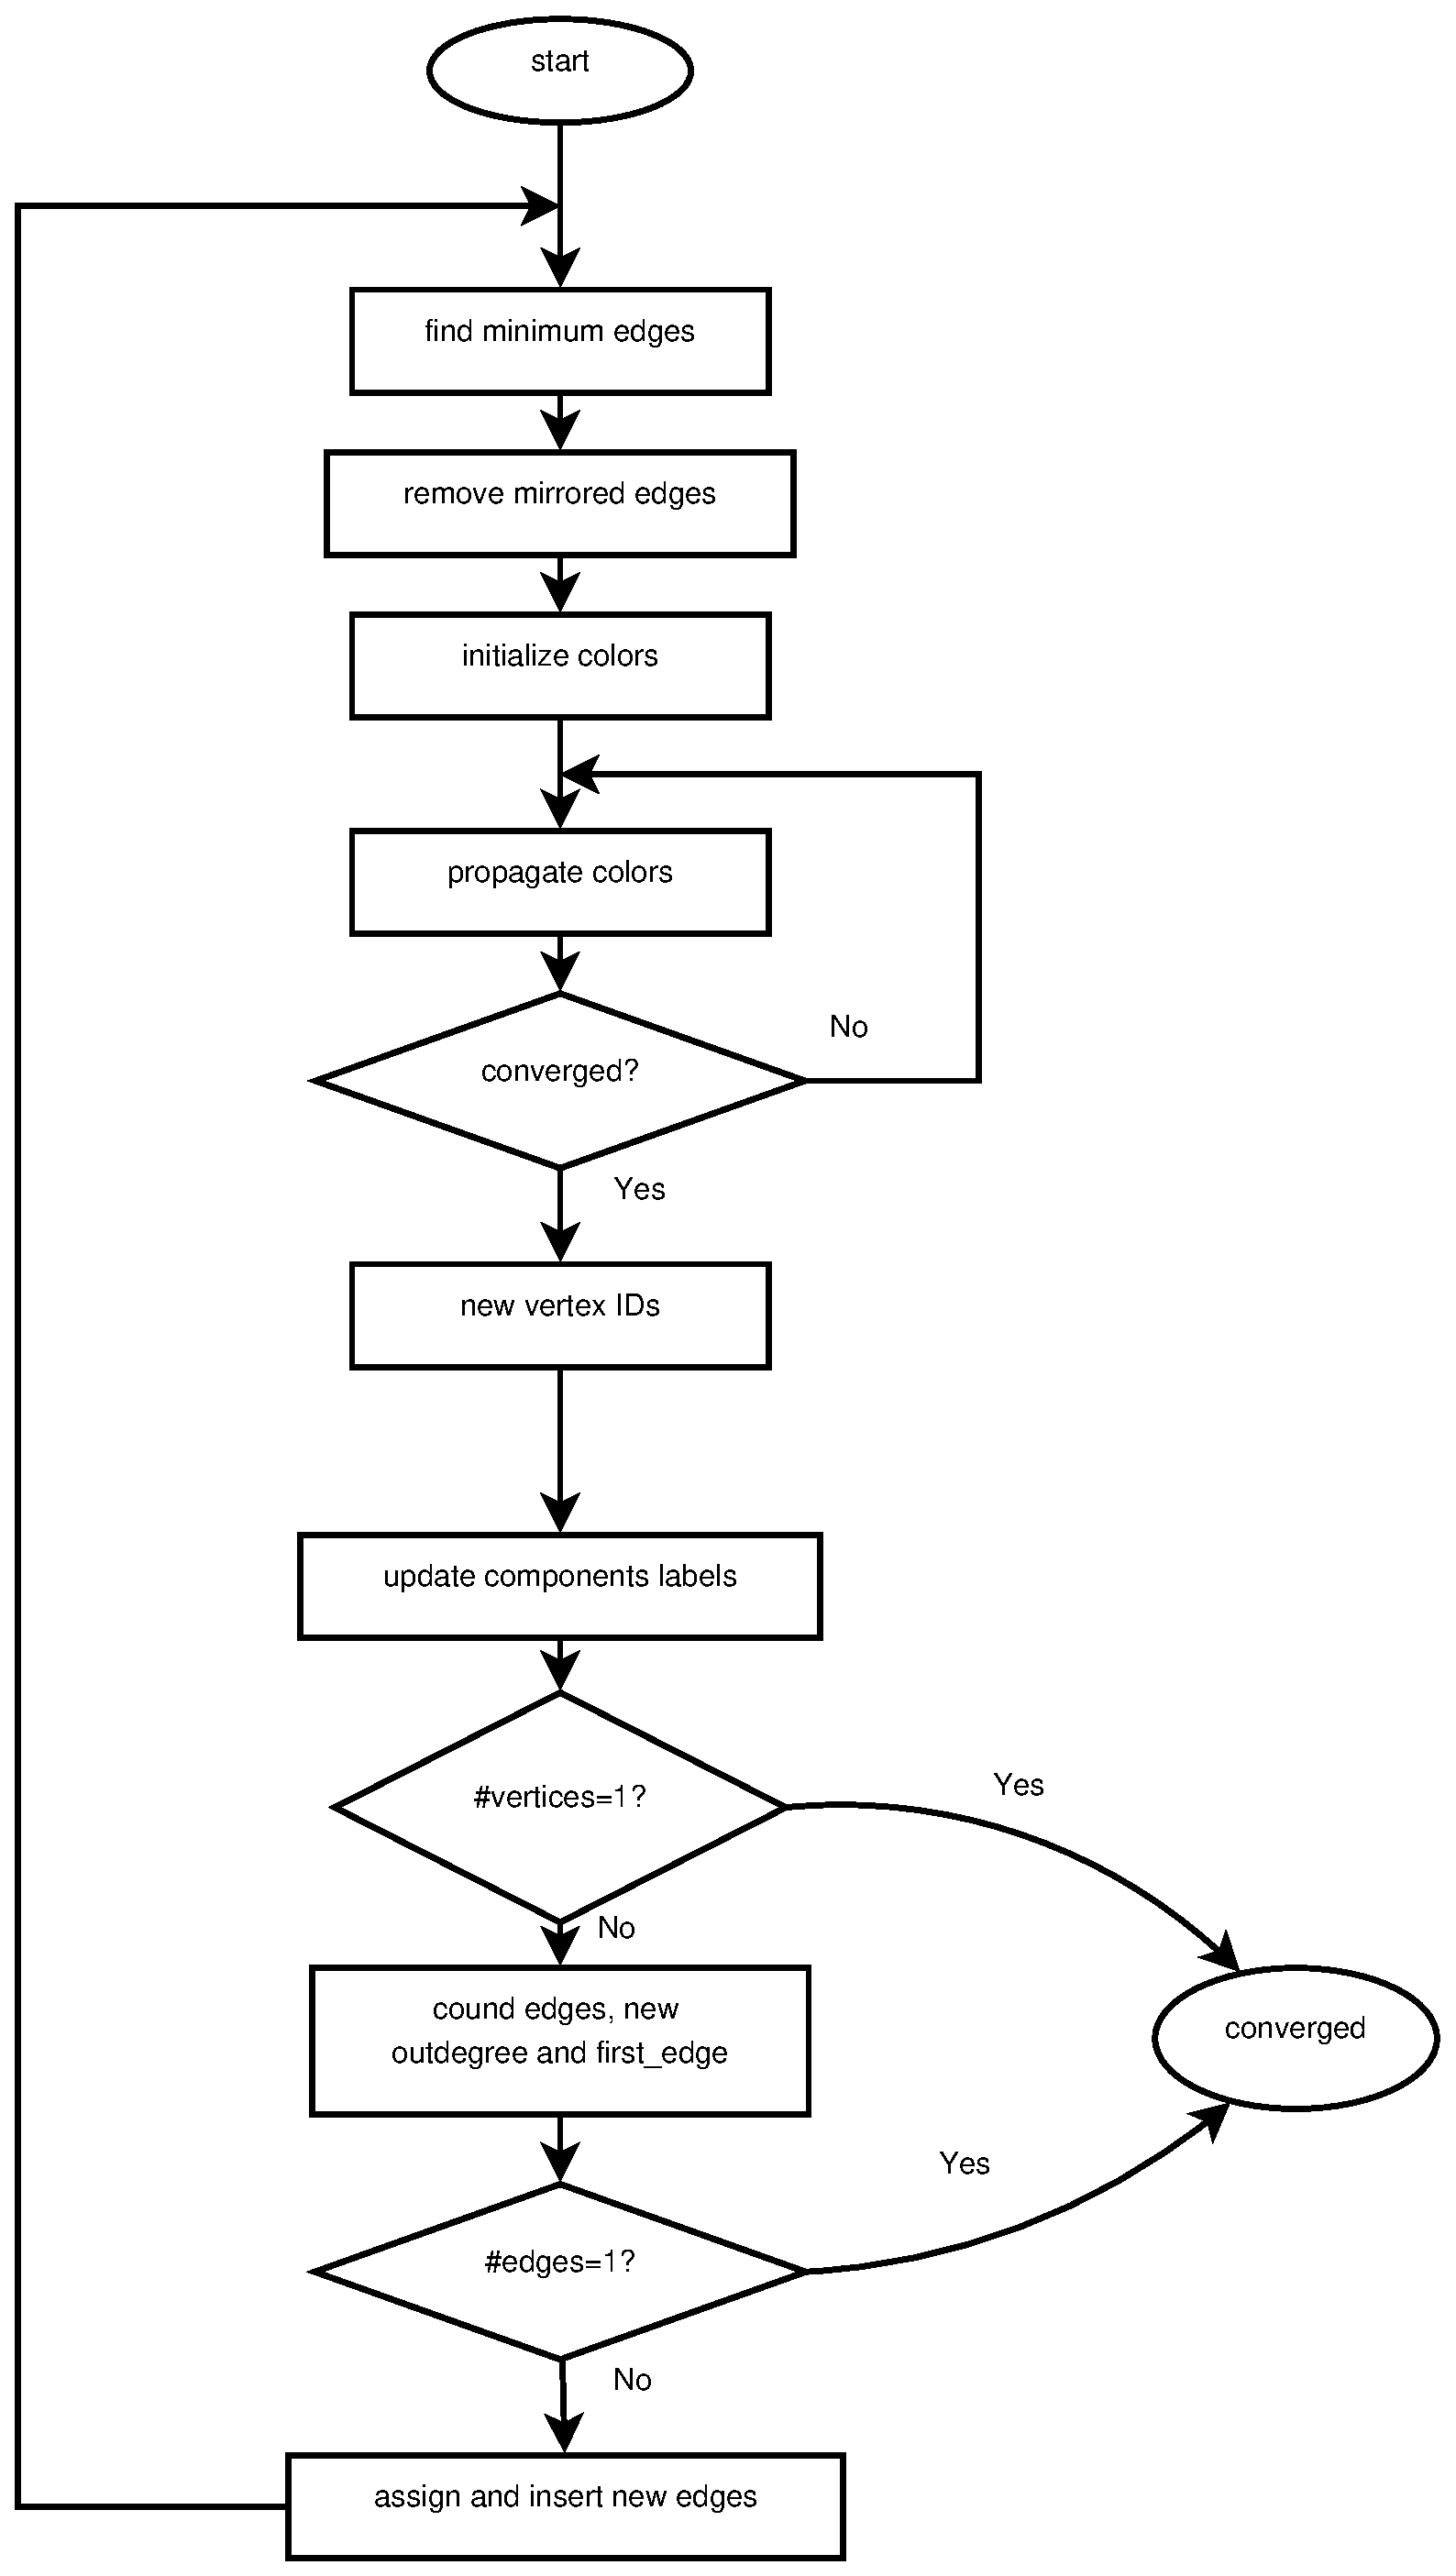
\includegraphics[scale=0.5]{methodology/connected_components_boruvka_flow.eps}
\caption{Diagram of the connected components labeling algorithm used.}
\label{fig:connected comps flow}
\end{figure}


%
% describe connected components algorithm
% how it copies colors in the first time
% and then just updates the labels with the new vertex IDs
%
% put flowchart and pseudocode


\begin{algorithm}
\caption{Update component labels kernel}\label{alg:comp_labels}
\begin{algorithmic}[1]
\Procedure{update\_labels}{$vertex\_id, labels, colors, new\_vertex$}
\State $curr\_color \gets labels[vertex\_id]$
\State $new\_color \gets colors[curr\_color]$
\State $new\_color\_id \gets new\_vertex[new\_color]$
\State $labels[vertex\_id] \gets new\_color\_id$
\EndProcedure
\end{algorithmic}
\end{algorithm}



\subsubsection{Memory transfer with the GPU}
The whole algorithm of computing the SL clustering has been implemented in the GPU with minimizing the memory utilization in mind.
Transferring the initial graph is the most relevant memory transfer.
It has to be transfered twice: first for computing the MST and then to build the processed MST graph.
This happens because the initial device arrays used for the graph are deallocated to give space for the arrays of subsequent iterations of the MST algorithm.
This implementation design had in mind memory consumption in mind and could easily be avoided with the cost of having to store the bigger initial graph for the entire duration of the MST computation, which might be worthwhile if the GPU memory is abundant.
The final labels array is transfered back to the host in the end of computation, but its size is small relative the to the size of the original graph.
Furthermore, because the control logic is processed by the host and it is dependent on some values computed by the device, extra memory transfers of single values (e.g. number of vertices and number of edges on each iteration) are necessary.
These, however, may be safely dismissed since they are of little consequence in the overall computation time.


\subsubsection{Contrast between implementations}

At this point it should be noted, for future reference, the contrast between the technology stack used by \citet{Sousa2015} and the one used here.
\citet{Sousa2015} used the native CUDA language to program the GPUs and highly optimized libraries.
The implementation in the present work used none of the above.
Accordingly, some performance may be lost.
This if specially true for some highly optimized operations that can be found in some libraries, since those use optimization mechanism that are not available in used CUDA API offered by the Numba package.
An evaluation of the interoperability between the technology stacks was made but, currently, this does not seem feasible.
Nevertheless, and whenever possible, we tried to close the gap so that these shortcomings become less noticeable in the overall performance.

\subsection{Single-Link and external memory algorithms}
\label{sec:sl disk}


The co-association matrix can become very large for large data sets.
Even using the EAC CSR method to reduce memory usage, the memory used occupy a significant portion of main memory.
Furthermore, the algorithm to compute a MST brings additional space complexity that make it infeasible to perform the final partition recovery on a large co-association matrix in main memory.
External memory algorithms address this issue.
% out of core processing %TODO check
External memory algorithms refers to algorithms that are based on disk (or other large capacity but typically low latency storage technology), usually by loading small batches to main memory, processing them, saving the results and repeat until the whole computation is done.
This section describes the process of building the MST with low memory usage.
The details of converting the MST in a Single-Link clustering are described in chapter \ref{chapter:stateofart} and omitted here.

\subsubsection{Kruskal's algorithm and implementation}

% Kruskal algorithm
The sequential MST algorithm used was Kruskal.
The original paper of Kruskal's \cite{kruskal1956shortest} algorithm describes three approaches for finding a MST.
The SciPy library offers an efficient implementation for the following construct (taken directly from the original paper of Kruskal's algorithm):
\begin{displayquote}
CONSTRUCTION A. Perform the following step as many times as possible: Among the edges of G not yet chosen, choose the shortest edge which does not form any loops with those edges already chosen. Clearly the set of edges eventually chosen must form a spanning tree of G, and in fact it forms a shortest spanning tree.
\end{displayquote}
If the graph if connected, the algorithm will stop before processing all edges when $|V| - 1$ edges are added to the MST.
Within the EAC context, it is very common for the co-association graph to have independent components which translates in every edge being processed.
It should be noted that this implementation works on a sparse matrix in the CSR format.

One of the main steps of the implementation is computing the order of the edges of the graph without sorting the edges themselves, an operation called \emph{argsort}.
To illustrate this, the argsort operation on the array $ \left [  4 , 5 , 2 , 1, 3 \right ]$ would yield $ \left [  3 , 2 , 4, 0 , 1 \right ]$ since the the smallest element is at position 3 (starting from 0), the second smalled at position 2, etc.
This operation is useful to avoid computing the edge with minimum (\emph{min}) weight in every iteration.
Doing so would increase time complexity since a sorting algorithm may have an average time complexity to $O(n log n)$ (QuickSort algorithm) while a single minimum has a time complexity of $O(n)$.
Computing the minimum at every iteration when every edge must be processed means that there will be $|E|$ iterations and so the total time complexity for the minimum operation alone will be $O(E ^ E)$ if processed edges are only given the maximum value possible or $O(E!)$ if they are removed.
These time complexities are much higher than a $O(E log E)$.
The result of this operation is an array of length $|E|$ (i.e. the number of associations in EAC), which means it will occupy at least the same size as the array containing the weights of the edges.
However, the total size is typically 8 times larger for EAC since the data type of the weights uses only one byte and the number of associations is very large, forcing a the use o 8 bytes for the argsort array.
This is the real motivation to store the co-association matrix in disk and use an external sorting algorithm.

\subsubsection{Kruskal's implementation with an external sorting algorithm}

The \emph{PyTables} library \cite{pytables}, which is built on top of the \emph{HDF5} format \cite{hdf5}, was used for storing the graph, performing the external sorting for the argsort operation and loading the graph in batches for processing.
This implementation starts by storing the CSR graph to disk.
However, instead of saving the \emph{indptr} array directly, an expanded version is stored instead.
The expanded version will be of the same length as the \emph{indices} array and the $i$-th element contains the origin vertex (or row) of the $i$-th edge.
This way, a binary search for discovering the origin vertex becomes unnecessary.

Afterwards, the argsort operation is performed by building a completely sorted index (CSI) of the \emph{data} array of the CSR matrix.
The details of CSI implementation fall outside the scope of this dissertation but are explained in further detail in \cite{AltetiAbad2007}.
It should be noted that the arrays themselves are not sorted.
Instead, the CSI allows for a fast indexing of the arrays in a sorted manner (according to the order of the edges).
%The CSI will be used to retrieve edges from the stored graph in a sorted manner.
The process of building the CSI has a very low main memory usage that can be disregarded.

The SciPy implementation of Kruskal's algorithm was modified to work with batches of the graph.
This was easily implemented just by making the additional data structures used in the building of MST persistent between calls of the function.
The new implementation loads the graph in batches and in a sorted manner, e.g. first load a batch of the 1000 smallest edges, then a batch of the next 1000 smalled edges, etc.
Each batch must be processed sequentially since the edges must be processed in a sorted manner, which means that there is no possibility for parallelism in this process.
Typically, the batch size is a very small fraction of the size of the edges, which means that the total memory usage for building the MST is overshadowed by the size of the co-association matrix.
The time complexity for building the CSI is higher that of computing the argsort operation, but the formal time complexity is not reported in the source \cite{AltetiAbad2007}.
As an example, for a 500000 pattern set the SL-MST approach took 54.9 seconds while the external memory approach took 2613.5 seconds - an order of magnitude higher.

\section{Resume of the developed work}

This chapter exposed a great deal of the actual developed work.
It covered solutions and implementations related to the three phases of EAC.
For the production of the ensemble, two quantum clustering algorithms and a GPU parallel K-Means variant were implemented.
These are algorithms existing in the literature (presented in chapter \ref{chapter:stateofart}) and implementation details were presented when relevant.
For addressing the computation complexity of the second phase of EAC, a novel method \textbf{EAC CSR} for building the co-association matrix was designed and implemented.
Finally, three approaches are presented for the last phase of EAC.
An implementation of a parallel GPU MST algorithm based on Borůvka's algorithm was presented along with a labeling algorithm for a forest of MSTs.
Also, an implementation of SL-MST based on Kruskal's algorithm and an external memory variant of it were presented.
The core of the external memory variant is based on using an external algorithm for sorting a very big array stored in disk and, although this is not something new, its application within the SL clustering framework was not found in literature.

% \subsubsection{Effects on the EAC algorithm}

% This section described two implementations for building a MST from a CSR graph.
% As mentioned before, using an MST based approach to Single-Link (SL-MST) already reduces significantly its computational complexity by only processing non-zero edges, which compose only a fraction of a co-association matrix in EAC.
% The implementation of SL-MST is based on the SciPy library and is explained above. 
% Still, the space complexity of MST-based SL can be too high for large data sets.
% This motivated the use of external algorithms using the PyTables library.
% The core concept of this approach is to store the co-association graph in disk and building a sorted index for later use.
% The sorted index is used for 



% \begin{tabular}{lrrr}
% \toprule
% % \hline
% {} &  threshold &   max\_assocs &  nnz percent relative to max \\
% \midrule
% % \hline
% 0  &   0.000000 &  1228.000000 &                     0.979769 \\
% 1  &   0.050000 &   794.000000 &                     0.613603 \\
% 2  &   0.100000 &   597.000000 &                     0.471318 \\
% 3  &   0.150000 &   496.000000 &                     0.386988 \\
% 4  &   0.200000 &   437.000000 &                     0.325645 \\
% 5  &   0.250000 &   367.000000 &                     0.276588 \\
% 6  &   0.300000 &   335.000000 &                     0.235490 \\
% 7  &   0.350000 &   294.000000 &                     0.200629 \\
% 8  &   0.400000 &   262.000000 &                     0.170249 \\
% 9  &   0.450000 &   232.000000 &                     0.143376 \\
% 10 &   0.500000 &   205.000000 &                     0.119374 \\
% 11 &   0.550000 &   167.000000 &                     0.098120 \\
% 12 &   0.600000 &   142.000000 &                     0.079426 \\
% 13 &   0.650000 &   121.000000 &                     0.062757 \\
% 14 &   0.700000 &   104.000000 &                     0.048278 \\
% 15 &   0.750000 &    88.000000 &                     0.035731 \\
% 16 &   0.800000 &    76.000000 &                     0.024967 \\
% 17 &   0.850000 &    68.000000 &                     0.015932 \\
% 18 &   0.900000 &    57.000000 &                     0.008913 \\
% 19 &   0.950000 &    38.000000 &                     0.003906 \\
% 20 &   0.000038 &     0.000086 &                     0.000046 \\
% \bottomrule
% % \hline
% \end{tabular}



\chapter{Final solution proposed}
\label{chapter:solution}

The final solution proposed is composed by the parallel K-Means implementation described, the EAC CSR method and the external memory variant for performing Single-Link.
The implementations have several parameters available for tinkering.
A general guideline of what is available and when should it be used is presented in this chapter.

It is recommended that the execution of the parallel K-Means algorithm be done with a "manual" memory transfer, so as to optimize GPU and host communication.
When the combined size of the data set, centroid set, labels and distance arrays exceed the available device memory, the pure sequential version of K-Means should be executed.
An optimized sequential version is offered alongside the implementation its parallel counterpart.

The choice of parameters of the method for building the co-association matrix is a simple one to make.
The available choices are:

\begin{itemize}
	\item if the matrix should be condensed (filling only the upper triangular) or not, 
	\item if the matrix should be sparse or not;
	\item within the sparse matrices, if a constant or linear memory allocation should be used.
\end{itemize}

The condensed version of the matrix is always preferred.
Not only does it occupy less than half of the memory, it also takes less time to build.
Furthermore, when this is paired with a sparse strategy, the final clustering is also nearly twice as fast.
A sparse representation should be chosen whenever $n (n-1) / 2$ times the size of the data type used (typically unsigned 1 byte integer) exceeds the available memory, where $n$ is the number of patterns in the data set.
The linear memory allocation is the ideal choice when a sparse representation of the condensed matrix is used, since half the memory is saved.

For the final clustering, the SLINK algorithm must be paired with a fully allocated matrix while the SL-MST strategy must be paired with a sparse representation.
Then, the final choice to make is if one should use the main memory approach for the final Single-Link clustering or the external memory approach.
Here, again, the decision is straightforward.
Typically if the sparse co-association matrix exceeds half of the available main memory, a external memory approach should be chosen.
The reason for this is that one of the crucial steps of the final clustering will almost double the memory used.